\textit{\underline{Raíces de un número complejo: }}

\begin{itemize}[label= \tiny \faIcon{meh}]

  \item \hypertarget{teoria-6:tablita}{Tablita de ángulos \textit{agradables}}:

        \begin{minipage}{0.5\textwidth}
          $$
            \begin{array}{|c|c|c|c|c|c|}
              \hline
                    \theta       & \red{0} & \color{orange}{\frac{\pi}{6}}      & \green{\frac{\pi}{4}}      & \color{blue}{\frac{\pi}{3}}      & \purple{\frac{\pi}{2}} \\ \hline
              \sin(\theta) & 0 & \frac{1}{2}        & \frac{\sqrt{2}}{2} & \frac{\sqrt{3}}{2} & 1             \\ \hline
              \cos(\theta) & 0 & \frac{\sqrt{3}}{2} & \frac{\sqrt{2}}{2} & \frac{1}{2}        & 1             \\ \hline
            \end{array}
          $$
                {\small
                \href{https://www.youtube.com/watch?v=83gdQe0Ij5k}{Clickea para está \textit{simpatética} forma de recordarlo:
                \purple{\faIcon{music}} um, dois, três, três, dois, um, todo mundo sobre 2...\purple{\faIcon{music}}}}
        \end{minipage}
        \begin{minipage}{0.5\textwidth}
          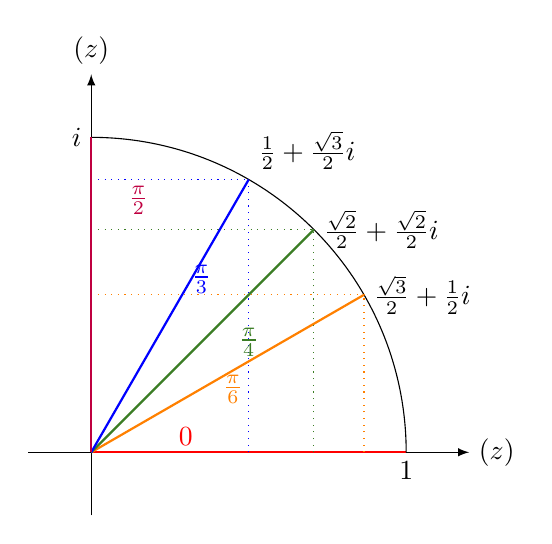
\begin{tikzpicture}[scale=4]
            % Draw the main coordinate axes
            \draw[-latex] (-0.2,0) -- (1.2,0) node[right] {$\re(z)$};
            \draw[-latex] (0,-0.2) -- (0,1.2) node[above] {$\im(z)$};

            \draw[red,thick] (0,0) -- (1,0);
            \draw[thin] (1,0) arc (0:90:1);

            \draw[orange,thick] (0,0) -- ({sqrt(3)/2},0.5);
            \draw[orange,dotted] ({sqrt(3)/2},0) -- ({sqrt(3)/2},0.5);
            \draw[orange,dotted] (0,0.5) -- ({sqrt(3)/2},0.5);

            \draw[OliveGreen,thick] (0,0) -- ({1/sqrt(2)},{1/sqrt(2)});
            \draw[OliveGreen,dotted] ({1/sqrt(2)},0) -- ({1/sqrt(2)},{1/sqrt(2)});
            \draw[OliveGreen,dotted] (0,{1/sqrt(2)}) -- ({1/sqrt(2)},{1/sqrt(2)});

            \draw[blue,thick] (0,0) -- (0.5,{sqrt(3)/2});
            \draw[blue,dotted] (0.5,0) -- (0.5,{sqrt(3)/2});
            \draw[blue,dotted] (0,{sqrt(3)/2}) -- (0.5,{sqrt(3)/2});

            \draw[purple,thick] (0,0) -- (0,1);

            \node[red] at (0.3,0.05) {$0$};
            \node[orange] at (0.45,0.2) {$\frac{\pi}{6}$};
            \node[OliveGreen] at (0.5,0.35) {$\frac{\pi}{4}$};
            \node[blue] at (0.35,0.55) {$\frac{\pi}{3}$};
            \node[purple] at (0.15,0.8) {$\frac{\pi}{2}$};

            \node[below] at (1,0) {$1$};
            \node[right] at ({sqrt(3)/2},0.5) {$\frac{\sqrt{3}}{2} + \frac{1}{2}i$};
            \node[right] at ({1/sqrt(2)},{1/sqrt(2)}) {$\frac{\sqrt{2}}{2} + \frac{\sqrt{2}}{2}i$};
            \node[above right] at (0.5,{sqrt(3)/2}) {$\frac{1}{2} + \frac{\sqrt{3}}{2}i$};
            \node[left] at (0,1) {$i$};
          \end{tikzpicture}
        \end{minipage}

  \item Sean $z, w \en \complejos -\set{0}$, $z = r_z e^{\theta_z i}$ y $w = r_w e^{\theta_w i }$ con $r_z,\, s_w \en \reales_{>0}$
        y $\theta_z,\, \theta_w \en \reales$.\par
        Entonces $z = w
          \Sii{\red{!!}}
          \llave{l}{
            r_z = r_w \\
            \theta_z = \theta_w + 2 k \pi,\ \text{para algún } k \en \enteros
          }$
  \item raíces $n$-esimas: $w^n = z
          \Sii{\red{!!}}
          \llave{l}{
            (r_w)^n = r_z \\
            \theta_w \cdot n = \theta_z + 2 k \pi \quad \text{para algún $k\en \enteros$}
          }$\par
        De donde se obtendrán $n$ raíces distintas:
        $$
          w_k = z_w e^{\theta_{w_k} i}, \text{ donde } r_w = \sqrt[n]{r_z} \ytext
          \theta_{w_k} = \frac{\theta_z}{n} + \frac{2k\pi}{n} = \frac{\theta_z + 2k\pi}{n}
        $$
        \red{Entender bien como sacar raíces $n$-ésimas es importantísimo para toda la guía de complejos y la próxima de polinomios}.
\end{itemize}

\underline{\textit{Grupos $G_n$:}}

\begin{itemize}[label=\color{gray} \tiny \faIcon{smile}]
\item $G_n = \set{w \en \complejos / w^n = 1} = \set{e^{\frac{2k \pi}{n} i}\ :\ 0\leq k \leq n-1}$
%==========================
% Macro para reducir los gráficos
\newcommand{\unitcircle}[1]{
  \begin{tikzpicture}[baseline=0, scale=1, every node/.style={font=\tiny}]
    \draw[ultra thin,->,gray] (-1.5,0) -- (1.8,0) node[below] {Re};
    \draw[ultra thin,->,gray] (0,-1.5) -- (0,1.5) node[right] {Im};
    \draw[ultra thin] (0,0) circle (1);
    \foreach \x in {0,...,#1} {
        \ifnum \x < #1 {
              \filldraw (\x*360/#1:0.8) node {$\x$};
              \filldraw (\x*360/#1:1) circle (1pt);
              \filldraw (\x*360/#1:1.4) node {$e^{i \frac{2\pi}{#1} \cdot \x}$};
              \draw[thick, Cerulean] (\x*360/#1:1) -- ({(\x+1)*360/#1}:1);
            }
        \fi
      }
  \end{tikzpicture}
}
% Fin macros
%================================

\begin{multicols}{2}
  \begin{enumerate}[label={($n$=\arabic*)}]
    \item $w = 1$
    \item $w = \pm 1$
    \item \unitcircle{3}
    \item \unitcircle{4}
    \item \unitcircle{5}
    \item \unitcircle{6}
    \item \unitcircle{7}
    \item \unitcircle{8}
    \item \unitcircle{9}
    \item \unitcircle{10}
  \end{enumerate}
\end{multicols}
Notar que:
\begin{itemize}
  \item Si $n$ es par el grupo tiene al $-1$.
  \item Toda raíz compleja tiene a su conjugado complejo.
  \item Para ir de un punto a otro, se lo múltiplica por $e^{i \theta}$ eso \textit{rota} al número en $\theta$
        respecto al origen.
\end{itemize}

\item $(G_n, \cdot)$ es un grupo abeliano, o conmutativo.
\begin{itemize}
  \item $\paratodo w, z \en G_n, w z = z  w \text{ y } z m \en G_n$.

  \item $1 \en G_n,\ w \cdot 1 = 1 \cdot w = w \qquad \paratodo w \en G_n$.

  \item $w \en G_n \entonces \existe w^{-1} \en G_n,\ w \cdot w^{-1} = w^{-1}\cdot w = 1$
        \begin{itemize}
          \item $\conj w \en G_n,\ w \cdot \conj w = |w|^2 = 1 \entonces \conj w = w^{-1}$
        \end{itemize}
\end{itemize}

\item \hypertarget{teoria6:propiedadesGn}{\textit{Propiedades: $w \en G_n$}}
\begin{itemize}
  \item $m \en \enteros$ y $n \divideA m \entonces w^m = 1$.

  \item $\congruencia{m}{m'}{n} \entonces w^m = w^{m'}\quad (w^m = w^{r_n(m)})$

  \item $n \divideA m \sisolosi G_n \subseteq G_m$

  \item $G_n \inter G_m = G_{(n:m)}$

  \item La suma de una raíz $w$ de $G_n$:
        $\sumatoria{k=0}{n-1}w^k = \frac{w^n -1}{w -1} = 0$ si $w \distinto 1$
\end{itemize}
